% Editable labelled graph; created for this workbench.
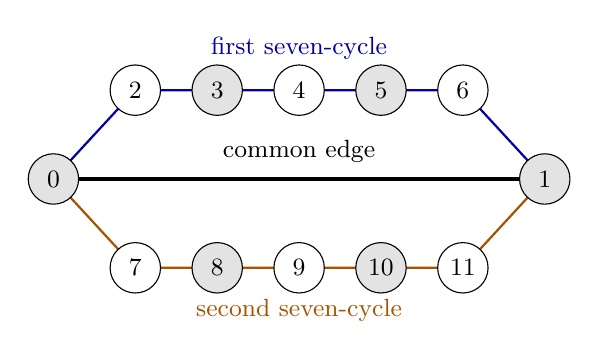
\begin{tikzpicture}[x=1.04cm,y=.94cm,
  vertex/.style={circle,draw=black,fill=white,minimum size=6.4mm,inner sep=1pt},
  chosen/.style={vertex,fill=gray!22},every node/.style={font=\small}]
\coordinate (a) at (0,0); \coordinate (b) at (6,0);
\foreach \i in {1,...,5} {
  \coordinate (p\i) at (\i,1.2);
  \coordinate (q\i) at (\i,-1.2);
}
\draw[very thick] (a)--node[above=2pt] {common edge} (b);
\draw[thick,blue!65!black] (a)--(p1)--(p2)--(p3)--(p4)--(p5)--(b);
\draw[thick,orange!65!black] (a)--(q1)--(q2)--(q3)--(q4)--(q5)--(b);
\node[chosen] at (a) {$0$}; \node[chosen] at (b) {$1$};
\foreach \i/\v in {1/2,3/4,5/6} {\node[vertex] at (p\i) {$\v$};}
\foreach \i/\v in {2/3,4/5} {\node[chosen] at (p\i) {$\v$};}
\foreach \i/\v in {1/7,3/9,5/11} {\node[vertex] at (q\i) {$\v$};}
\foreach \i/\v in {2/8,4/10} {\node[chosen] at (q\i) {$\v$};}
\node[blue!65!black] at (3,1.77) {first seven-cycle};
\node[orange!65!black] at (3,-1.77) {second seven-cycle};
\end{tikzpicture}
